\documentclass[14pt]{extbook}
\usepackage{multicol, enumerate, enumitem, hyperref, color, soul, setspace, parskip, fancyhdr} %General Packages
\usepackage{amssymb, amsthm, amsmath, latexsym, units, mathtools} %Math Packages
\everymath{\displaystyle} %All math in Display Style
% Packages with additional options
\usepackage[headsep=0.5cm,headheight=12pt, left=1 in,right= 1 in,top= 1 in,bottom= 1 in]{geometry}
\usepackage[usenames,dvipsnames]{xcolor}
\usepackage{dashrule}  % Package to use the command below to create lines between items
\newcommand{\litem}[1]{\item#1\hspace*{-1cm}\rule{\textwidth}{0.4pt}}
\pagestyle{fancy}
\lhead{Progress Quiz 10}
\chead{}
\rhead{Version ALL}
\lfoot{5170-5105}
\cfoot{}
\rfoot{Summer C 2021}
\begin{document}

\begin{enumerate}
\litem{
Which of the following equations \textit{could} be of the graph presented below?
\begin{center}
    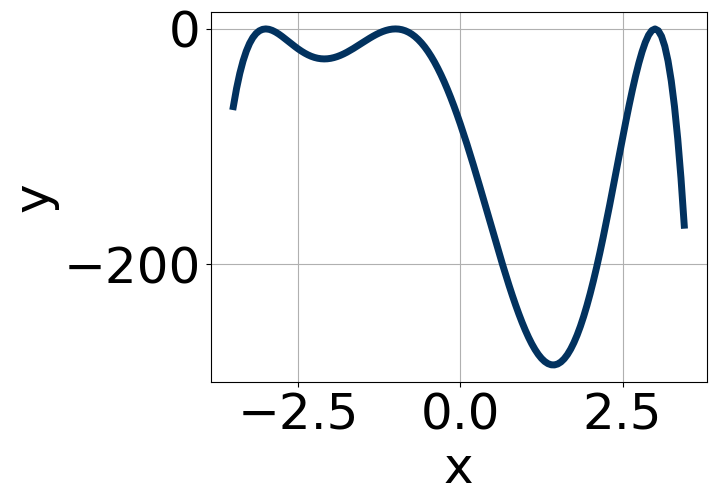
\includegraphics[width=0.5\textwidth]{../Figures/polyGraphToFunctionA.png}
\end{center}
\begin{enumerate}[label=\Alph*.]
\item \( -18(x + 3)^{6} (x + 1)^{4} (x - 3)^{8} \)
\item \( 12(x + 3)^{8} (x + 1)^{4} (x - 3)^{7} \)
\item \( -7(x + 3)^{6} (x + 1)^{10} (x - 3)^{7} \)
\item \( 8(x + 3)^{6} (x + 1)^{6} (x - 3)^{6} \)
\item \( -12(x + 3)^{10} (x + 1)^{11} (x - 3)^{5} \)

\end{enumerate} }
\litem{
Describe the end behavior of the polynomial below.\[ f(x) = -9(x + 8)^{2}(x - 8)^{5}(x - 6)^{2}(x + 6)^{3} \]\begin{enumerate}[label=\Alph*.]
\begin{multicols}{2}\item 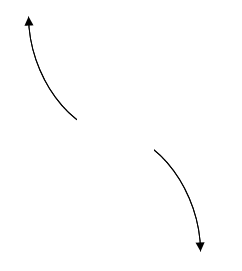
\includegraphics[width = 0.3\textwidth]{../Figures/polyEndBehaviorAA.png}\item 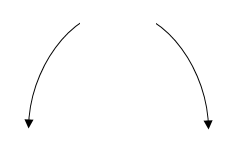
\includegraphics[width = 0.3\textwidth]{../Figures/polyEndBehaviorBA.png}\item 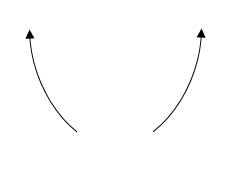
\includegraphics[width = 0.3\textwidth]{../Figures/polyEndBehaviorCA.png}\item 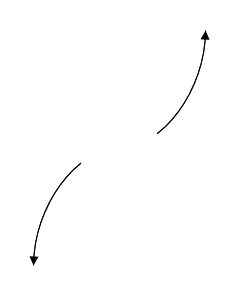
\includegraphics[width = 0.3\textwidth]{../Figures/polyEndBehaviorDA.png}\end{multicols}\item None of the above.
\end{enumerate} }
\litem{
Construct the lowest-degree polynomial given the zeros below. Then, choose the intervals that contain the coefficients of the polynomial in the form $x^3+bx^2+cx+d$.\[ 4 + 3 i \text{ and } 1 \]\begin{enumerate}[label=\Alph*.]
\item \( b \in [1, 2], c \in [-6, -4.35], \text{ and } d \in [3.48, 4.06] \)
\item \( b \in [1, 2], c \in [-4.24, -2.63], \text{ and } d \in [2.96, 3.37] \)
\item \( b \in [-17, -7], c \in [31.51, 33.82], \text{ and } d \in [-25.2, -24.86] \)
\item \( b \in [8, 10], c \in [31.51, 33.82], \text{ and } d \in [24.44, 25.5] \)
\item \( \text{None of the above.} \)

\end{enumerate} }
\litem{
Which of the following equations \textit{could} be of the graph presented below?
\begin{center}
    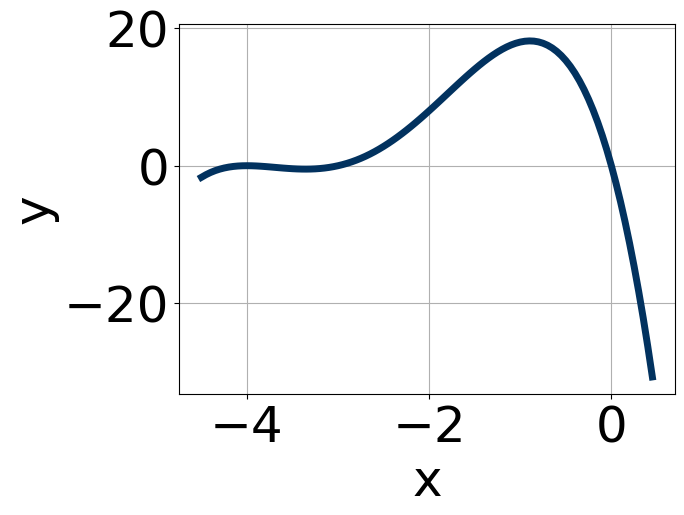
\includegraphics[width=0.5\textwidth]{../Figures/polyGraphToFunctionCopyA.png}
\end{center}
\begin{enumerate}[label=\Alph*.]
\item \( -5x^{5} (x + 4)^{8} (x + 3)^{7} \)
\item \( -19x^{6} (x + 4)^{6} (x + 3)^{7} \)
\item \( -14x^{10} (x + 4)^{9} (x + 3)^{5} \)
\item \( 10x^{11} (x + 4)^{8} (x + 3)^{10} \)
\item \( 19x^{11} (x + 4)^{4} (x + 3)^{7} \)

\end{enumerate} }
\litem{
Describe the zero behavior of the zero $x = 8$ of the polynomial below.\[ f(x) = -9(x - 6)^{9}(x + 6)^{6}(x - 8)^{12}(x + 8)^{9} \]\begin{enumerate}[label=\Alph*.]
\begin{multicols}{2}\item 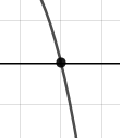
\includegraphics[width = 0.3\textwidth]{../Figures/polyZeroBehaviorCopyAA.png}\item 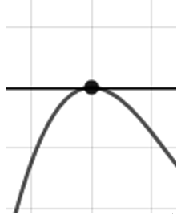
\includegraphics[width = 0.3\textwidth]{../Figures/polyZeroBehaviorCopyBA.png}\item 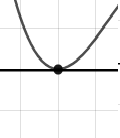
\includegraphics[width = 0.3\textwidth]{../Figures/polyZeroBehaviorCopyCA.png}\item 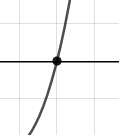
\includegraphics[width = 0.3\textwidth]{../Figures/polyZeroBehaviorCopyDA.png}\end{multicols}\item None of the above.
\end{enumerate} }
\litem{
Construct the lowest-degree polynomial given the zeros below. Then, choose the intervals that contain the coefficients of the polynomial in the form $ax^3+bx^2+cx+d$.\[ \frac{3}{2}, 5, \text{ and } \frac{-4}{3} \]\begin{enumerate}[label=\Alph*.]
\item \( a \in [0, 10], b \in [45, 52], c \in [97, 103], \text{ and } d \in [55, 64] \)
\item \( a \in [0, 10], b \in [-34, -27], c \in [-9, -4], \text{ and } d \in [55, 64] \)
\item \( a \in [0, 10], b \in [-34, -27], c \in [-9, -4], \text{ and } d \in [-66, -56] \)
\item \( a \in [0, 10], b \in [26, 37], c \in [-9, -4], \text{ and } d \in [-66, -56] \)
\item \( a \in [0, 10], b \in [-13, -7], c \in [-76, -68], \text{ and } d \in [-66, -56] \)

\end{enumerate} }
\litem{
Construct the lowest-degree polynomial given the zeros below. Then, choose the intervals that contain the coefficients of the polynomial in the form $x^3+bx^2+cx+d$.\[ -3 + 2 i \text{ and } 2 \]\begin{enumerate}[label=\Alph*.]
\item \( b \in [-5.5, -1.2], c \in [-3, 3], \text{ and } d \in [24, 27] \)
\item \( b \in [0.7, 1.5], c \in [-6, -3], \text{ and } d \in [0, 9] \)
\item \( b \in [3.8, 5.3], c \in [-3, 3], \text{ and } d \in [-32, -24] \)
\item \( b \in [0.7, 1.5], c \in [-3, 3], \text{ and } d \in [-10, -3] \)
\item \( \text{None of the above.} \)

\end{enumerate} }
\litem{
Construct the lowest-degree polynomial given the zeros below. Then, choose the intervals that contain the coefficients of the polynomial in the form $ax^3+bx^2+cx+d$.\[ \frac{-3}{5}, \frac{-7}{2}, \text{ and } \frac{-3}{2} \]\begin{enumerate}[label=\Alph*.]
\item \( a \in [15, 23], b \in [110, 119], c \in [165, 169], \text{ and } d \in [-64, -58] \)
\item \( a \in [15, 23], b \in [-117, -109], c \in [165, 169], \text{ and } d \in [-64, -58] \)
\item \( a \in [15, 23], b \in [110, 119], c \in [165, 169], \text{ and } d \in [54, 68] \)
\item \( a \in [15, 23], b \in [-53, -49], c \in [-85, -80], \text{ and } d \in [54, 68] \)
\item \( a \in [15, 23], b \in [88, 93], c \in [36, 51], \text{ and } d \in [-64, -58] \)

\end{enumerate} }
\litem{
Describe the zero behavior of the zero $x = 7$ of the polynomial below.\[ f(x) = 2(x + 7)^{7}(x - 7)^{10}(x - 3)^{4}(x + 3)^{8} \]\begin{enumerate}[label=\Alph*.]
\begin{multicols}{2}\item 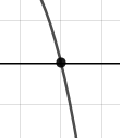
\includegraphics[width = 0.3\textwidth]{../Figures/polyZeroBehaviorAA.png}\item 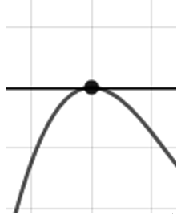
\includegraphics[width = 0.3\textwidth]{../Figures/polyZeroBehaviorBA.png}\item 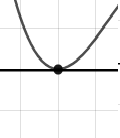
\includegraphics[width = 0.3\textwidth]{../Figures/polyZeroBehaviorCA.png}\item 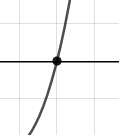
\includegraphics[width = 0.3\textwidth]{../Figures/polyZeroBehaviorDA.png}\end{multicols}\item None of the above.
\end{enumerate} }
\litem{
Describe the end behavior of the polynomial below.\[ f(x) = -3(x + 4)^{3}(x - 4)^{6}(x - 5)^{5}(x + 5)^{7} \]\begin{enumerate}[label=\Alph*.]
\begin{multicols}{2}\item 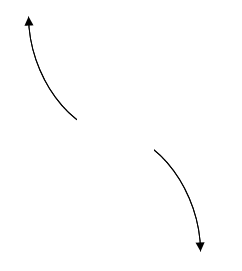
\includegraphics[width = 0.3\textwidth]{../Figures/polyEndBehaviorCopyAA.png}\item 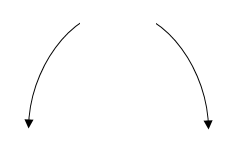
\includegraphics[width = 0.3\textwidth]{../Figures/polyEndBehaviorCopyBA.png}\item 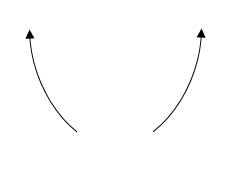
\includegraphics[width = 0.3\textwidth]{../Figures/polyEndBehaviorCopyCA.png}\item 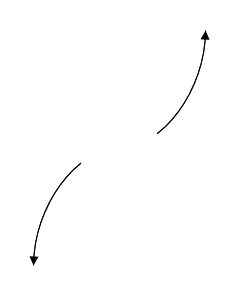
\includegraphics[width = 0.3\textwidth]{../Figures/polyEndBehaviorCopyDA.png}\end{multicols}\item None of the above.
\end{enumerate} }
\litem{
Which of the following equations \textit{could} be of the graph presented below?
\begin{center}
    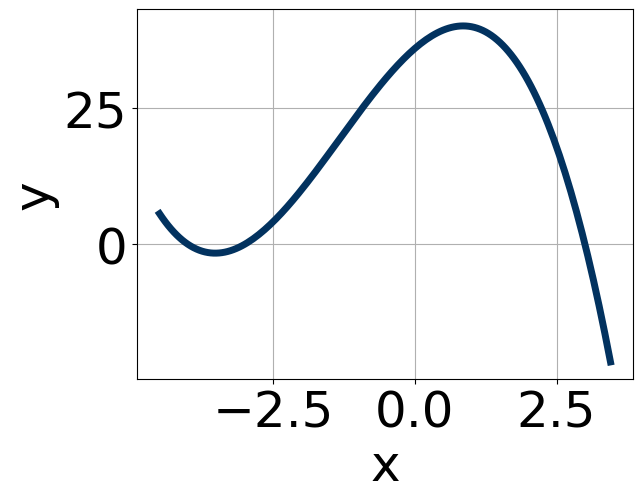
\includegraphics[width=0.5\textwidth]{../Figures/polyGraphToFunctionB.png}
\end{center}
\begin{enumerate}[label=\Alph*.]
\item \( -20(x - 3)^{6} (x + 4)^{11} (x + 3)^{5} \)
\item \( -3(x - 3)^{7} (x + 4)^{9} (x + 3)^{11} \)
\item \( 6(x - 3)^{4} (x + 4)^{11} (x + 3)^{9} \)
\item \( -3(x - 3)^{4} (x + 4)^{8} (x + 3)^{9} \)
\item \( 18(x - 3)^{5} (x + 4)^{5} (x + 3)^{11} \)

\end{enumerate} }
\litem{
Describe the end behavior of the polynomial below.\[ f(x) = 6(x + 4)^{5}(x - 4)^{6}(x - 3)^{4}(x + 3)^{5} \]\begin{enumerate}[label=\Alph*.]
\begin{multicols}{2}\item 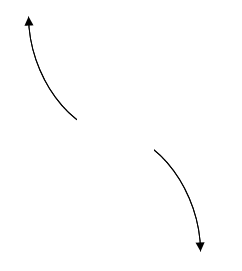
\includegraphics[width = 0.3\textwidth]{../Figures/polyEndBehaviorAB.png}\item 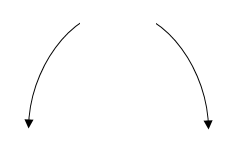
\includegraphics[width = 0.3\textwidth]{../Figures/polyEndBehaviorBB.png}\item 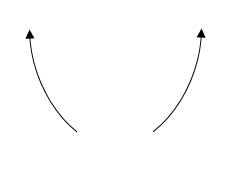
\includegraphics[width = 0.3\textwidth]{../Figures/polyEndBehaviorCB.png}\item 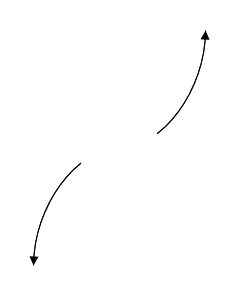
\includegraphics[width = 0.3\textwidth]{../Figures/polyEndBehaviorDB.png}\end{multicols}\item None of the above.
\end{enumerate} }
\litem{
Construct the lowest-degree polynomial given the zeros below. Then, choose the intervals that contain the coefficients of the polynomial in the form $x^3+bx^2+cx+d$.\[ -5 + 5 i \text{ and } -3 \]\begin{enumerate}[label=\Alph*.]
\item \( b \in [-1, 9], c \in [-8, 1], \text{ and } d \in [-15, -11] \)
\item \( b \in [11, 16], c \in [80, 82], \text{ and } d \in [147, 158] \)
\item \( b \in [-1, 9], c \in [7, 11], \text{ and } d \in [11, 19] \)
\item \( b \in [-19, -12], c \in [80, 82], \text{ and } d \in [-158, -146] \)
\item \( \text{None of the above.} \)

\end{enumerate} }
\litem{
Which of the following equations \textit{could} be of the graph presented below?
\begin{center}
    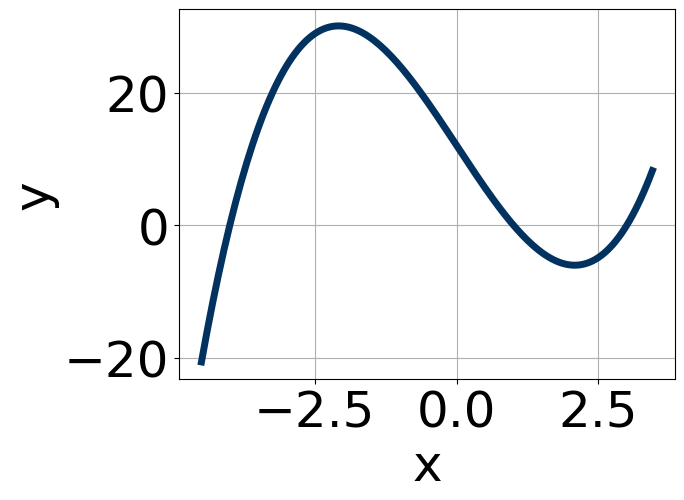
\includegraphics[width=0.5\textwidth]{../Figures/polyGraphToFunctionCopyB.png}
\end{center}
\begin{enumerate}[label=\Alph*.]
\item \( 3(x - 3)^{4} (x + 4)^{8} (x - 1)^{5} \)
\item \( -12(x - 3)^{4} (x + 4)^{5} (x - 1)^{7} \)
\item \( 9(x - 3)^{7} (x + 4)^{11} (x - 1)^{11} \)
\item \( -12(x - 3)^{9} (x + 4)^{11} (x - 1)^{5} \)
\item \( 10(x - 3)^{6} (x + 4)^{11} (x - 1)^{7} \)

\end{enumerate} }
\litem{
Describe the zero behavior of the zero $x = -8$ of the polynomial below.\[ f(x) = 9(x + 2)^{11}(x - 2)^{7}(x + 8)^{7}(x - 8)^{6} \]\begin{enumerate}[label=\Alph*.]
\begin{multicols}{2}\item 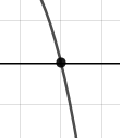
\includegraphics[width = 0.3\textwidth]{../Figures/polyZeroBehaviorCopyAB.png}\item 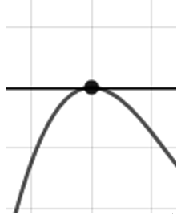
\includegraphics[width = 0.3\textwidth]{../Figures/polyZeroBehaviorCopyBB.png}\item 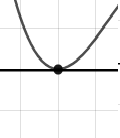
\includegraphics[width = 0.3\textwidth]{../Figures/polyZeroBehaviorCopyCB.png}\item 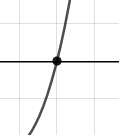
\includegraphics[width = 0.3\textwidth]{../Figures/polyZeroBehaviorCopyDB.png}\end{multicols}\item None of the above.
\end{enumerate} }
\litem{
Construct the lowest-degree polynomial given the zeros below. Then, choose the intervals that contain the coefficients of the polynomial in the form $ax^3+bx^2+cx+d$.\[ \frac{5}{2}, \frac{-1}{3}, \text{ and } \frac{-2}{3} \]\begin{enumerate}[label=\Alph*.]
\item \( a \in [17, 23], b \in [19, 28], c \in [-45, -36], \text{ and } d \in [8, 11] \)
\item \( a \in [17, 23], b \in [-27, -24], c \in [-45, -36], \text{ and } d \in [-17, -9] \)
\item \( a \in [17, 23], b \in [50, 54], c \in [3, 12], \text{ and } d \in [-17, -9] \)
\item \( a \in [17, 23], b \in [58, 75], c \in [44, 53], \text{ and } d \in [8, 11] \)
\item \( a \in [17, 23], b \in [-27, -24], c \in [-45, -36], \text{ and } d \in [8, 11] \)

\end{enumerate} }
\litem{
Construct the lowest-degree polynomial given the zeros below. Then, choose the intervals that contain the coefficients of the polynomial in the form $x^3+bx^2+cx+d$.\[ 4 + 5 i \text{ and } -2 \]\begin{enumerate}[label=\Alph*.]
\item \( b \in [1, 3], c \in [-4.5, -2.7], \text{ and } d \in [-10.1, -9.4] \)
\item \( b \in [1, 3], c \in [-2.53, -1.56], \text{ and } d \in [-8.9, -6.6] \)
\item \( b \in [6, 11], c \in [22.96, 25.33], \text{ and } d \in [-83.9, -75.9] \)
\item \( b \in [-7, -3], c \in [22.96, 25.33], \text{ and } d \in [80.5, 82.2] \)
\item \( \text{None of the above.} \)

\end{enumerate} }
\litem{
Construct the lowest-degree polynomial given the zeros below. Then, choose the intervals that contain the coefficients of the polynomial in the form $ax^3+bx^2+cx+d$.\[ \frac{7}{5}, \frac{-1}{4}, \text{ and } \frac{2}{5} \]\begin{enumerate}[label=\Alph*.]
\item \( a \in [97, 103], b \in [75, 77], c \in [-81, -77], \text{ and } d \in [6, 19] \)
\item \( a \in [97, 103], b \in [-163, -151], c \in [5, 14], \text{ and } d \in [-14, -13] \)
\item \( a \in [97, 103], b \in [-163, -151], c \in [5, 14], \text{ and } d \in [6, 19] \)
\item \( a \in [97, 103], b \in [147, 156], c \in [5, 14], \text{ and } d \in [-14, -13] \)
\item \( a \in [97, 103], b \in [119, 127], c \in [-37, -25], \text{ and } d \in [-14, -13] \)

\end{enumerate} }
\litem{
Describe the zero behavior of the zero $x = -6$ of the polynomial below.\[ f(x) = 9(x - 6)^{5}(x + 6)^{10}(x - 9)^{7}(x + 9)^{11} \]\begin{enumerate}[label=\Alph*.]
\begin{multicols}{2}\item 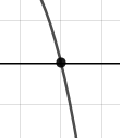
\includegraphics[width = 0.3\textwidth]{../Figures/polyZeroBehaviorAB.png}\item 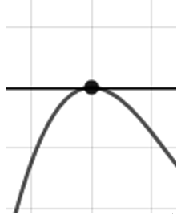
\includegraphics[width = 0.3\textwidth]{../Figures/polyZeroBehaviorBB.png}\item 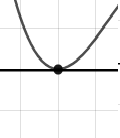
\includegraphics[width = 0.3\textwidth]{../Figures/polyZeroBehaviorCB.png}\item 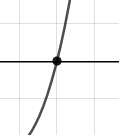
\includegraphics[width = 0.3\textwidth]{../Figures/polyZeroBehaviorDB.png}\end{multicols}\item None of the above.
\end{enumerate} }
\litem{
Describe the end behavior of the polynomial below.\[ f(x) = -8(x - 2)^{4}(x + 2)^{5}(x + 9)^{5}(x - 9)^{6} \]\begin{enumerate}[label=\Alph*.]
\begin{multicols}{2}\item 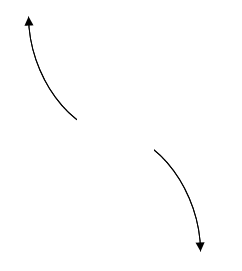
\includegraphics[width = 0.3\textwidth]{../Figures/polyEndBehaviorCopyAB.png}\item 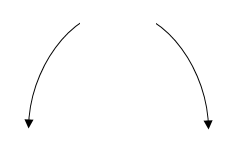
\includegraphics[width = 0.3\textwidth]{../Figures/polyEndBehaviorCopyBB.png}\item 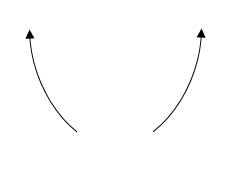
\includegraphics[width = 0.3\textwidth]{../Figures/polyEndBehaviorCopyCB.png}\item 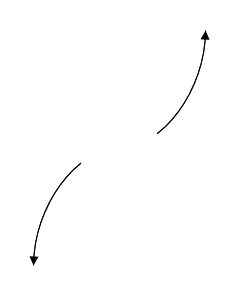
\includegraphics[width = 0.3\textwidth]{../Figures/polyEndBehaviorCopyDB.png}\end{multicols}\item None of the above.
\end{enumerate} }
\litem{
Which of the following equations \textit{could} be of the graph presented below?
\begin{center}
    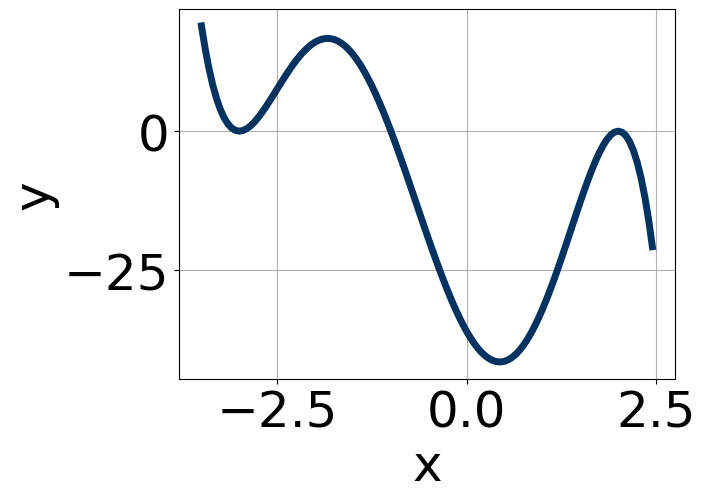
\includegraphics[width=0.5\textwidth]{../Figures/polyGraphToFunctionC.png}
\end{center}
\begin{enumerate}[label=\Alph*.]
\item \( 19(x - 2)^{10} (x + 3)^{6} (x + 1)^{8} \)
\item \( -18(x - 2)^{10} (x + 3)^{6} (x + 1)^{11} \)
\item \( -19(x - 2)^{8} (x + 3)^{9} (x + 1)^{10} \)
\item \( 13(x - 2)^{10} (x + 3)^{10} (x + 1)^{5} \)
\item \( -4(x - 2)^{10} (x + 3)^{5} (x + 1)^{5} \)

\end{enumerate} }
\litem{
Describe the end behavior of the polynomial below.\[ f(x) = 4(x + 6)^{4}(x - 6)^{9}(x + 9)^{3}(x - 9)^{3} \]\begin{enumerate}[label=\Alph*.]
\begin{multicols}{2}\item 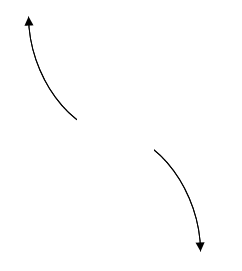
\includegraphics[width = 0.3\textwidth]{../Figures/polyEndBehaviorAC.png}\item 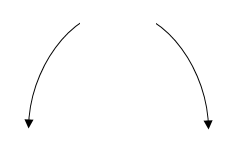
\includegraphics[width = 0.3\textwidth]{../Figures/polyEndBehaviorBC.png}\item 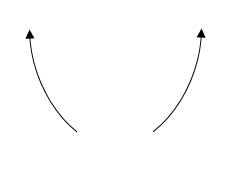
\includegraphics[width = 0.3\textwidth]{../Figures/polyEndBehaviorCC.png}\item 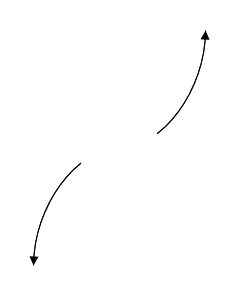
\includegraphics[width = 0.3\textwidth]{../Figures/polyEndBehaviorDC.png}\end{multicols}\item None of the above.
\end{enumerate} }
\litem{
Construct the lowest-degree polynomial given the zeros below. Then, choose the intervals that contain the coefficients of the polynomial in the form $x^3+bx^2+cx+d$.\[ -3 - 5 i \text{ and } -4 \]\begin{enumerate}[label=\Alph*.]
\item \( b \in [-1, 5], c \in [8, 9.7], \text{ and } d \in [16, 22] \)
\item \( b \in [-1, 5], c \in [6.7, 8.6], \text{ and } d \in [10, 14] \)
\item \( b \in [-15, -8], c \in [56.1, 58.3], \text{ and } d \in [-143, -134] \)
\item \( b \in [6, 14], c \in [56.1, 58.3], \text{ and } d \in [130, 141] \)
\item \( \text{None of the above.} \)

\end{enumerate} }
\litem{
Which of the following equations \textit{could} be of the graph presented below?
\begin{center}
    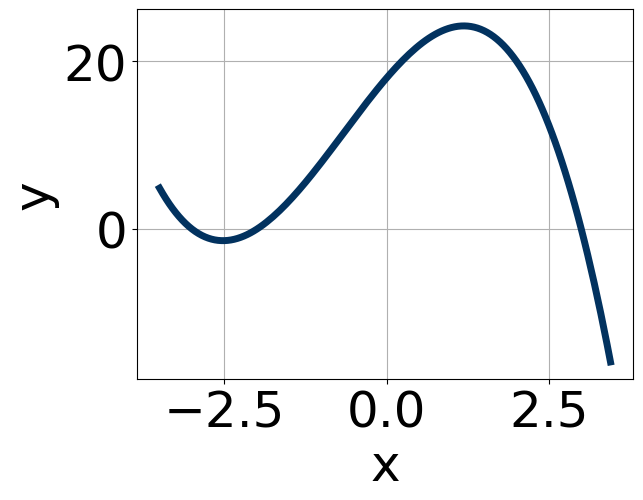
\includegraphics[width=0.5\textwidth]{../Figures/polyGraphToFunctionCopyC.png}
\end{center}
\begin{enumerate}[label=\Alph*.]
\item \( 7(x + 2)^{6} (x + 3)^{11} (x - 3)^{7} \)
\item \( -10(x + 2)^{10} (x + 3)^{9} (x - 3)^{9} \)
\item \( 11(x + 2)^{9} (x + 3)^{9} (x - 3)^{9} \)
\item \( -2(x + 2)^{9} (x + 3)^{11} (x - 3)^{5} \)
\item \( -5(x + 2)^{4} (x + 3)^{8} (x - 3)^{9} \)

\end{enumerate} }
\litem{
Describe the zero behavior of the zero $x = -6$ of the polynomial below.\[ f(x) = -9(x - 6)^{9}(x + 6)^{10}(x + 2)^{9}(x - 2)^{12} \]\begin{enumerate}[label=\Alph*.]
\begin{multicols}{2}\item 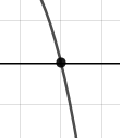
\includegraphics[width = 0.3\textwidth]{../Figures/polyZeroBehaviorCopyAC.png}\item 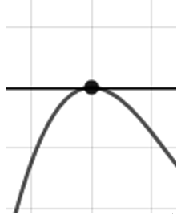
\includegraphics[width = 0.3\textwidth]{../Figures/polyZeroBehaviorCopyBC.png}\item 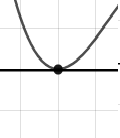
\includegraphics[width = 0.3\textwidth]{../Figures/polyZeroBehaviorCopyCC.png}\item 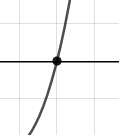
\includegraphics[width = 0.3\textwidth]{../Figures/polyZeroBehaviorCopyDC.png}\end{multicols}\item None of the above.
\end{enumerate} }
\litem{
Construct the lowest-degree polynomial given the zeros below. Then, choose the intervals that contain the coefficients of the polynomial in the form $ax^3+bx^2+cx+d$.\[ -2, \frac{-7}{3}, \text{ and } \frac{3}{2} \]\begin{enumerate}[label=\Alph*.]
\item \( a \in [5, 11], b \in [16, 20], c \in [-14, -9], \text{ and } d \in [40, 47] \)
\item \( a \in [5, 11], b \in [-12, -2], c \in [-33, -27], \text{ and } d \in [40, 47] \)
\item \( a \in [5, 11], b \in [-43, -32], c \in [63, 68], \text{ and } d \in [-47, -37] \)
\item \( a \in [5, 11], b \in [-21, -14], c \in [-14, -9], \text{ and } d \in [40, 47] \)
\item \( a \in [5, 11], b \in [16, 20], c \in [-14, -9], \text{ and } d \in [-47, -37] \)

\end{enumerate} }
\litem{
Construct the lowest-degree polynomial given the zeros below. Then, choose the intervals that contain the coefficients of the polynomial in the form $x^3+bx^2+cx+d$.\[ -4 - 3 i \text{ and } -3 \]\begin{enumerate}[label=\Alph*.]
\item \( b \in [11, 19], c \in [48.36, 49.78], \text{ and } d \in [72.6, 77.1] \)
\item \( b \in [0, 7], c \in [4.02, 6.83], \text{ and } d \in [7.9, 9.5] \)
\item \( b \in [0, 7], c \in [6.29, 9.06], \text{ and } d \in [11.8, 14.7] \)
\item \( b \in [-16, -10], c \in [48.36, 49.78], \text{ and } d \in [-76, -71.8] \)
\item \( \text{None of the above.} \)

\end{enumerate} }
\litem{
Construct the lowest-degree polynomial given the zeros below. Then, choose the intervals that contain the coefficients of the polynomial in the form $ax^3+bx^2+cx+d$.\[ \frac{-7}{5}, \frac{-1}{4}, \text{ and } \frac{3}{5} \]\begin{enumerate}[label=\Alph*.]
\item \( a \in [100, 104], b \in [-230, -224], c \in [129, 136], \text{ and } d \in [-21, -15] \)
\item \( a \in [100, 104], b \in [-177, -171], c \in [30, 38], \text{ and } d \in [20, 32] \)
\item \( a \in [100, 104], b \in [-112, -104], c \in [-65, -60], \text{ and } d \in [20, 32] \)
\item \( a \in [100, 104], b \in [103, 115], c \in [-65, -60], \text{ and } d \in [20, 32] \)
\item \( a \in [100, 104], b \in [103, 115], c \in [-65, -60], \text{ and } d \in [-21, -15] \)

\end{enumerate} }
\litem{
Describe the zero behavior of the zero $x = 7$ of the polynomial below.\[ f(x) = -7(x - 3)^{11}(x + 3)^{9}(x - 7)^{14}(x + 7)^{9} \]\begin{enumerate}[label=\Alph*.]
\begin{multicols}{2}\item 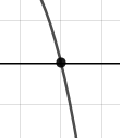
\includegraphics[width = 0.3\textwidth]{../Figures/polyZeroBehaviorAC.png}\item 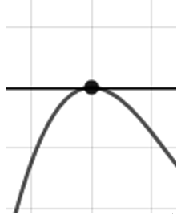
\includegraphics[width = 0.3\textwidth]{../Figures/polyZeroBehaviorBC.png}\item 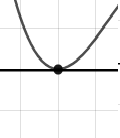
\includegraphics[width = 0.3\textwidth]{../Figures/polyZeroBehaviorCC.png}\item 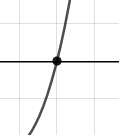
\includegraphics[width = 0.3\textwidth]{../Figures/polyZeroBehaviorDC.png}\end{multicols}\item None of the above.
\end{enumerate} }
\litem{
Describe the end behavior of the polynomial below.\[ f(x) = -3(x + 9)^{5}(x - 9)^{8}(x - 3)^{2}(x + 3)^{3} \]\begin{enumerate}[label=\Alph*.]
\begin{multicols}{2}\item \includegraphics[width = 0.3\textwidth]{../Figures/polyEndBehaviorCopyAC.png}\item \includegraphics[width = 0.3\textwidth]{../Figures/polyEndBehaviorCopyBC.png}\item \includegraphics[width = 0.3\textwidth]{../Figures/polyEndBehaviorCopyCC.png}\item \includegraphics[width = 0.3\textwidth]{../Figures/polyEndBehaviorCopyDC.png}\end{multicols}\item None of the above.
\end{enumerate} }
\end{enumerate}

\end{document}